\section{Реализация инструмента для анализа обменов на шине I2C}

В рамках курсовой работы стояла задача по реализации инструмента для анализа обменов на шине I2C на базе уже существующего решения для визуализации и анализа обменов Opermon. В этом разделе описаны детали реализации решения.

\subsection{Исследование предметной области}

\subsubsection{Устройство шины I2C}

I2C [\ref{i2c_protocol_spec}] — последовательная шина данных для связи интегральных схем, использующая две двунаправленные линии связи. Используется для соединения низкоскоростных периферийных компонентов с материнской платой, встраиваемыми системами и мобильными телефонами. Название представляет собой аббревиатуру слов Inter-Integrated Circuit. Шина данных поддерживает ``горячее'' подключение устройств (без перезапуска всей системы), а также одновременную работу нескольких ведущих устройств.

Данные передаются по двум проводам — \textit{линии данных} (SDA) и \textit{линии тактов} (SCL). В обмене всегда участвует два устройства: ведущий (\textit{master}) и ведомый (\textit{slave}). Тактовый сигнал на линии SCL генерируется ведущим устройством; ведомое устройство использует этот сигнал как опорный в том числе и для передачи данных к ведущему. Всего на одной двупроводной шине может быть до 127 устройств (адрес ведомого устройства кодируется 7 битами данных).

Каждая линия подключена к ``плюсу'' питания устройства через специальный \textit{подтягивающий резистор}. Таким образом, когда шина свободна  (обмены не производятся), с обеих линий считывается высокий уровень напряжения (логическая единица). Когда устройство начинает передачу, оно подключает требуемую линию к ``минусу'' питания и на линии устанавливается низкий уровень напряжения (логический ноль). Такая схема подключения называется \textit{монтажное ``И''}. Она позволяет нескольким устройствам устанавливать уровни одновременно без риска образования короткого замыкания и, как следствие, повреждения устройств.

Обмен начинается с события \textbf{START}, когда ведущее устройство устанавливает низкий уровень на линии данных (SDA) при высоком уровне на линии тактирования (SCL). В этот момент остальные устройства на линии определяют шину как занятую и ожидают окончания передачи.

После события \textbf{START} ведущее устройство передаёт байт, содержащий адрес ведомого устройства (7 бит) и бит режим обмена: 1 (R) - получение данных от ведомого устройства (чтение), 0 (W) - передача данных ведомому устройству (запись). Если на линии есть устройство с указанным адресом, оно должно установить линию SDA в низкий уровень для подтверждения приёма (событие \textbf{ACK}, от англ. acknowledge - подтверждение).

После этого происходит непосредственно обмен данными: в зависимости от выбранного режима, либо данные передаются от ведомого устройства, либо от ведущего. Получатель должен подтверждать приём каждого байта (исключение делается только для последнего байта в режиме чтения данных - master должен сообщить ведомому устройству об окончании приёма). Тактовый сигнал генерируется ведущим устройством, но при необходимости ведомое устройство может устанавливать тактовую линию в низкий уровень и, таким образом, задерживать обмен (например, если не успевает обрабатывать данные).

В конце обмена ведущее устройство меняет состояние линии SDA с низкого на высокий при высоком уровне на линии SCL - событие \textbf{STOP}. После этого шина считается освобождённой и в ней могут начинаться новые обмены.

\begin{figure}[H]
 \centering
 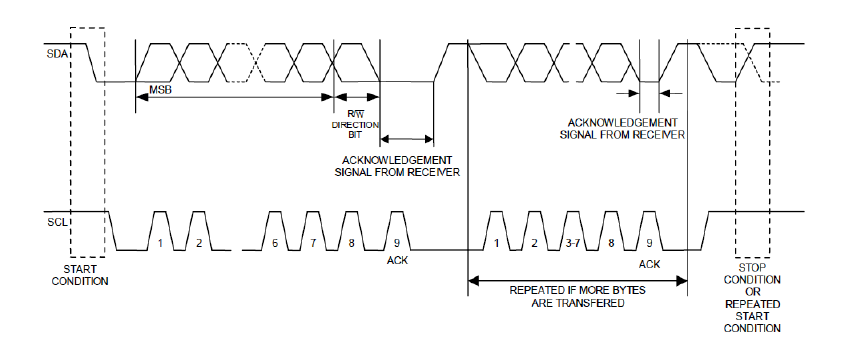
\includegraphics[width=\textwidth]{i2c_exchange}
 \caption{Структура информационного обмена на шине I2C}
 \label{fig:i2c_exchange}
\end{figure}

Таким образом, для представления корректного обмена мы можем получить следующую информацию:

\begin{itemize}
 \item \textbf{Время начала обмена} - время возникновения события \textbf{START};
 \item \textbf{Длительность обмена} - время между событиями \textbf{START} и \textbf{STOP};
 \item Адрес ведомого устройства;
 \item Режим передачи - R или W;
 \item Передаваемые данные (полезная нагрузка, payload).
\end{itemize}

Обмен может содержать ошибки. Следующие ошибки могут быть обнаружены на этапе считывания обмена:

\begin{itemize}
 \item Ведомое устройство не найдено - отсутствует ACK после первого байта обмена;
 \item Ведомое устройство потеряно или неисправно - отсутствует ACK после переданного байта;
 \item Некорректное начало передачи - отсутствует событие START.
\end{itemize}

\subsubsection{Выбор адаптера}

Для получения данных с шины I2C был выбран адаптер Bus Pirate [\ref{buspirate_descr}] по следующим причинам:

\begin{enumerate}
 \item Адаптер имеет простой и удобный интерфейс взаимодействия, как консольный (для работы без специализированного ПО), так и бинарный;
 \item Bus Pirate поддерживает режим I2C sniffer [\ref{buspirate_i2c}], что необходимо для реализации средства анализа;
 \item Bus Pirate - проект с открытым исходным кодом и открытой реализацией оборудования. Вокруг проекта образовалось обширное сообщество, постоянно занимающееся разработкой новых версий аппаратного и программного обеспечения;
 \item Доступная стоимость адаптера.
\end{enumerate}

Сообщения в формате Bus Pirate имеют текстовый формат. Данные об обменах представляются в следующем виде [\ref{buspirate_i2c_snif}]:

\begin{itemize}
 \item символ ``\textbf{[}'' обозначает начало обмена (событие \textbf{START});
 \item символ ``\textbf{]}'' обозначает конец сообщения (событие \textbf{STOP});
 \item ответы принимающей стороны - \textbf{ACK} и \textbf{NACK} кодируются символами ``\textbf{+}'' и ``\textbf{-}'' соответственно;
 \item передаваемые данные начинаются с символа ``\textbf{\textbackslash}'', после чего идёт шестнадцатеричное представление байта в виде 0x$NM$, где $N$, $M$ - шестнадцатеричные цифры (от 0 до F).
\end{itemize}

Пример фрагмента получаемого потока данных от адаптера:

\begin{verbatim}
 [ \0xA0+ \0x01+ \0x02+ ] [ \0xA1+ \0xDE+ \0xAD+ \0xF0+ \0x0D- ]
\end{verbatim}

\subsection{Проектирование решения}

\subsubsection{Серверная часть}

Задача удалённого агента - определять подключенные к системе совместимые адаптеры и осуществлять обмен данными между Opermon и выбранным адаптером. Обмен с адаптером происходит посредством последовательного соединения.

Алгоритм поиска доступных в системе адаптеров приведён на схеме ниже. С помощью такого алгоритма можно определить также устройства, совместимые с Bus Pirate. При проверке адаптер только переводится в режим бинарного интерфейса, что безопасно для подключенного оборудования. После проверки обнаруженные адаптеры перезапускаются для того, чтобы оставить пользователю возможность использовать часть адаптеров в режиме консольного интерфейса.

\begin{figure}[H]
 \centering
 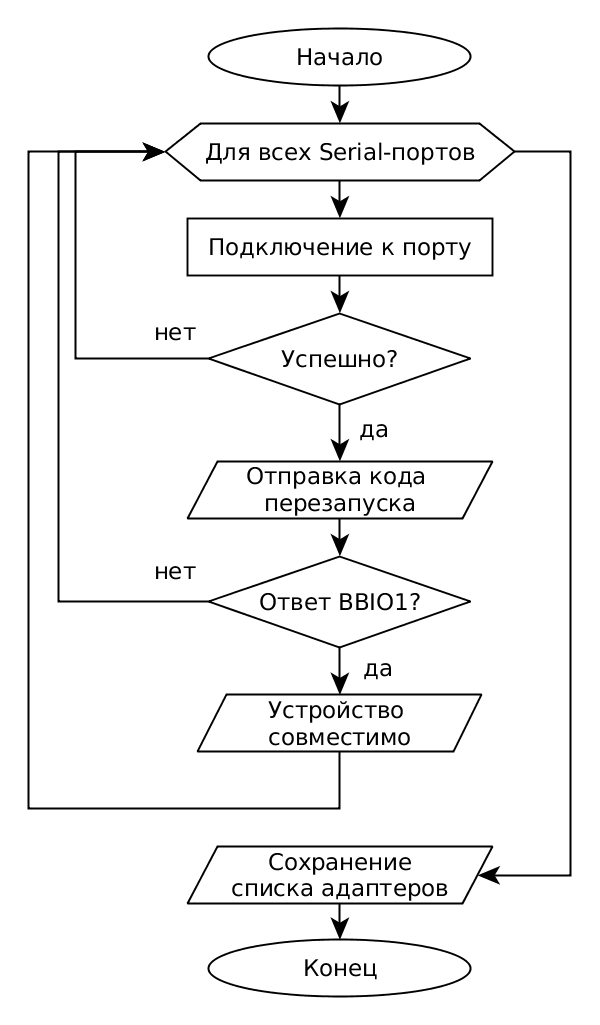
\includegraphics[width=0.5\textwidth]{bp-discovery}
 \caption{Алгоритм обнаружения Bus Pirate - совместимых адаптеров в системе}
 \label{fig:bp-discovery}
\end{figure}

Добавление нового адаптера в серверную часть означает следующую последовательность действий:

\begin{enumerate}
 \item добавление класса (C++), соответствующего типу адаптера, а также реализация в нём методов для управления адаптером, список которых приведён в разделе \ref{agent_proc_list};
 \item добавление создания экземпляра класса и вызовов методов в процедуру обработки RPC-запросов;
 \item реализация процедуры получения и сериализации данных от адаптера для передачи их клиентской части.
\end{enumerate}

\subsubsection{Клиентская часть}

В клиентской части требуется проводить разбор сообщений из данных, приходящих от Bus Pirate, во внутренние представления Opermon, а также реализовать необходимые виджеты для отображения данных и настройки параметров. 

Добавление нового типа адаптера в Opermon означает следующую последовательность действий:

\begin{enumerate}
 \item описание нового типа обменов в компоненте Tabexchange;
 \item описание нового типа представления адаптера в клиентской части;
 \item реализация процедуры получения данных от серверной части и создание экземпляров нового типа обменов на их базе;
 \item добавление создания экземпляра класса представления адаптера в соответствующую процедуру в Opermon;
 \item реализация необходимых для работы виджетов на базе предлагаемых в решении интерфейсов в компоненте sma;
 \item добавление создания экземпляров классов виджетов и код для их базовой настройки в фабрику виджетов.
\end{enumerate}


\subsection{Добавление поддержки адаптера в Opermon}

\subsubsection{Серверная часть}

Серверная часть решения реализована с использованием библиотеки QSerialPort [\ref{qtserialport}] для упрощения работы с последовательным интерфесом адаптера.

Для реализации поддержки адаптера на стороне сервера были выполнены следующие действия:

\begin{enumerate}
 \item создана обёртка для библиотеки QSerialPort для сборки в рамках системы сборки cvslvk;
 \item в файлах opermon/agent/buspirate.cpp и opermon/agent/buspirate.h описан класс BusPirate представления адаптера, наследуемый от класса CommonCard, и реализованы методы для инициализации, конфигурирования и обмена данными с представлением адаптера посредством RPC;
 \item в файле opermon/agent/rpcserver.cpp в обработчик RPC-запросов RpcServer::processRequest() добавлено создание объекта представления адаптера и вызовы соответствующих методов;
 \item в opermon/agent/Makefile добавлено правило для сборки новых файлов, а также добавлена зависимость от QSerialPort.
\end{enumerate}


\subsubsection{Клиентская часть}




Снимок экрана с окном получившегося интерфейса можно посмотреть в приложении \ref{app:figures} на рисунке \ref{fig:opermon}.